\section{SP-сети. Проект «Люцифер»}\label{section-project-lucifer}\index{шифр!«Люцифер»|(}
\selectlanguage{russian}

В 1973 году в "Scientific American" появляется статья сотрудника IBM (а ранее -- ВМС США) Хорста Фейстеля (\langen{Horst Feistel}) <<Cryptography and Computer Privacy>>~\cite{Feistel:1973}, описывающая проект функции шифрования <<Люцифер>>, который можно считать прообразом современных блочных шифров. Развитием данной системы стал государственный стандарт США <<Digital Encryption Standard>> с 1979 по 2001 годы.

\begin{figure}[!t]
    \centering
    \subfloat[$S$-блок. На вход поступает 3 бита информации, которые трактуются как двоичное представление номера одной из $2^3$ линий внутреннего $P$-блока. На выходе номер активной сигнальной дорожки обратно преобразуется в 3-битовое представление]{\label{fig:s-box-inside} 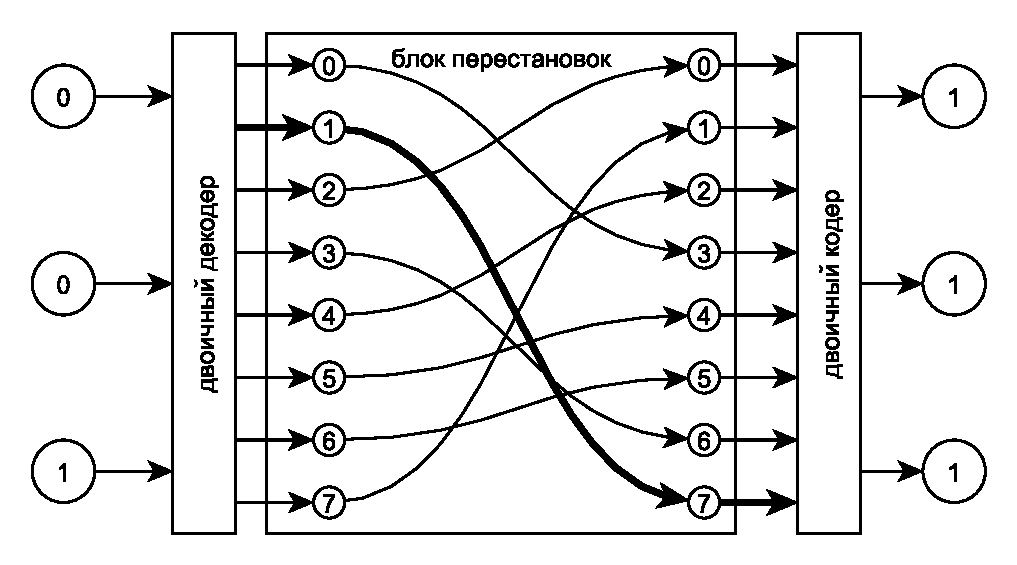
\includegraphics[width=0.66\textwidth]{pic/s-box-inside}}
    ~~~
    \subfloat[P-блок. Все поступающие на вход биты не меняются, но перемешиваются внутри блока]{\label{fig:p-box-inside} 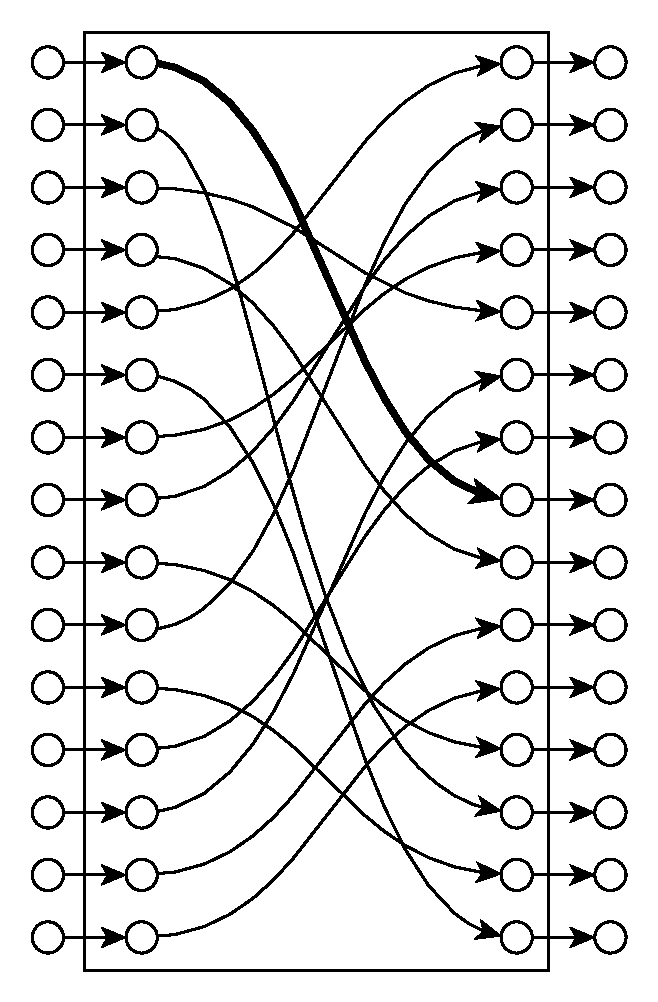
\includegraphics[width=0.25\textwidth]{pic/p-box-inside}}
		\caption{Возможные реализации $S$- и $P$-блоков}
\end{figure}

Фейстель высказывает идею, что идеальный шифр для блока размером в 128 бит должен включать в себя блок замен (substitution box, $S$-box, далее $S$-блок), который мог бы обработать сразу 128 бит входного блока данных. $S$-блок принимает на вход блок бит и даёт на выходе другой блок бит (возможно, даже другого размера) согласно некоторому словарю или результату вычисления нелинейной функции\footnote{Нелинейная функция в целях производительности также может быть технологически реализована в виде выборки уже вычисленного значения по аргументу из словаря.}. К сожалению, физическая реализация (см. рис.~\ref{fig:s-box-inside}) действительно произвольного блока замен для входа в 128 бит потребовала бы $2^{128}$ внутренних соединений, либо словаря из $2^{128}$ 128-битовых значений, если реализовывать программным способом, что технологически невозможно\footnote{Причём в шифре таких блоков должно быть столько же, сколько разных ключей мог бы иметь шифр.}. Зато если такой блок можно было бы создать, то он был бы очень хорош с криптографической точки зрения. Даже если криптоаналитик знает произвольное число пар значений вход-выход, это ничего не скажет ему об остальном множестве значений. То есть без полного перебора всех возможных $2^{128}$ вариантов входа криптоаналитик не сможет составить полное представление о внутренней структуре блока.

С другой стороны, блок перестановок (permutation box, $P$-box, далее $P$-блок), как изображённый на рис.~\ref{fig:p-box-inside}, может обрабатывать блоки битов любого размера. Однако какая-либо криптографическая стойкость у него отсутствует: он представляет собой тривиальное линейное преобразование своего входа. Криптоаналитику достаточно иметь $N$ линейно независимых пар значений входа и выхода (где $N$ -- размер блока), чтобы получить полное представление о структуре P-блока.

\index{SP-сеть|(}
Идея Фейстеля состояла в том, чтобы комбинировать $S$- и $P$-блоки, позволяя на практике получить большой блок нелинейных преобразований (то есть один большой $S$-блок), как изображено на рис.~\ref{fig:sp-network}. При достаточном числе <<слоёв>> $SP$-сеть начинает обладать свойствами хорошего $S$-блока (сложность криптографического анализа и выявления структуры), при этом оставаясь технологически простой в реализации.

\begin{figure}[htb]
	\centering
	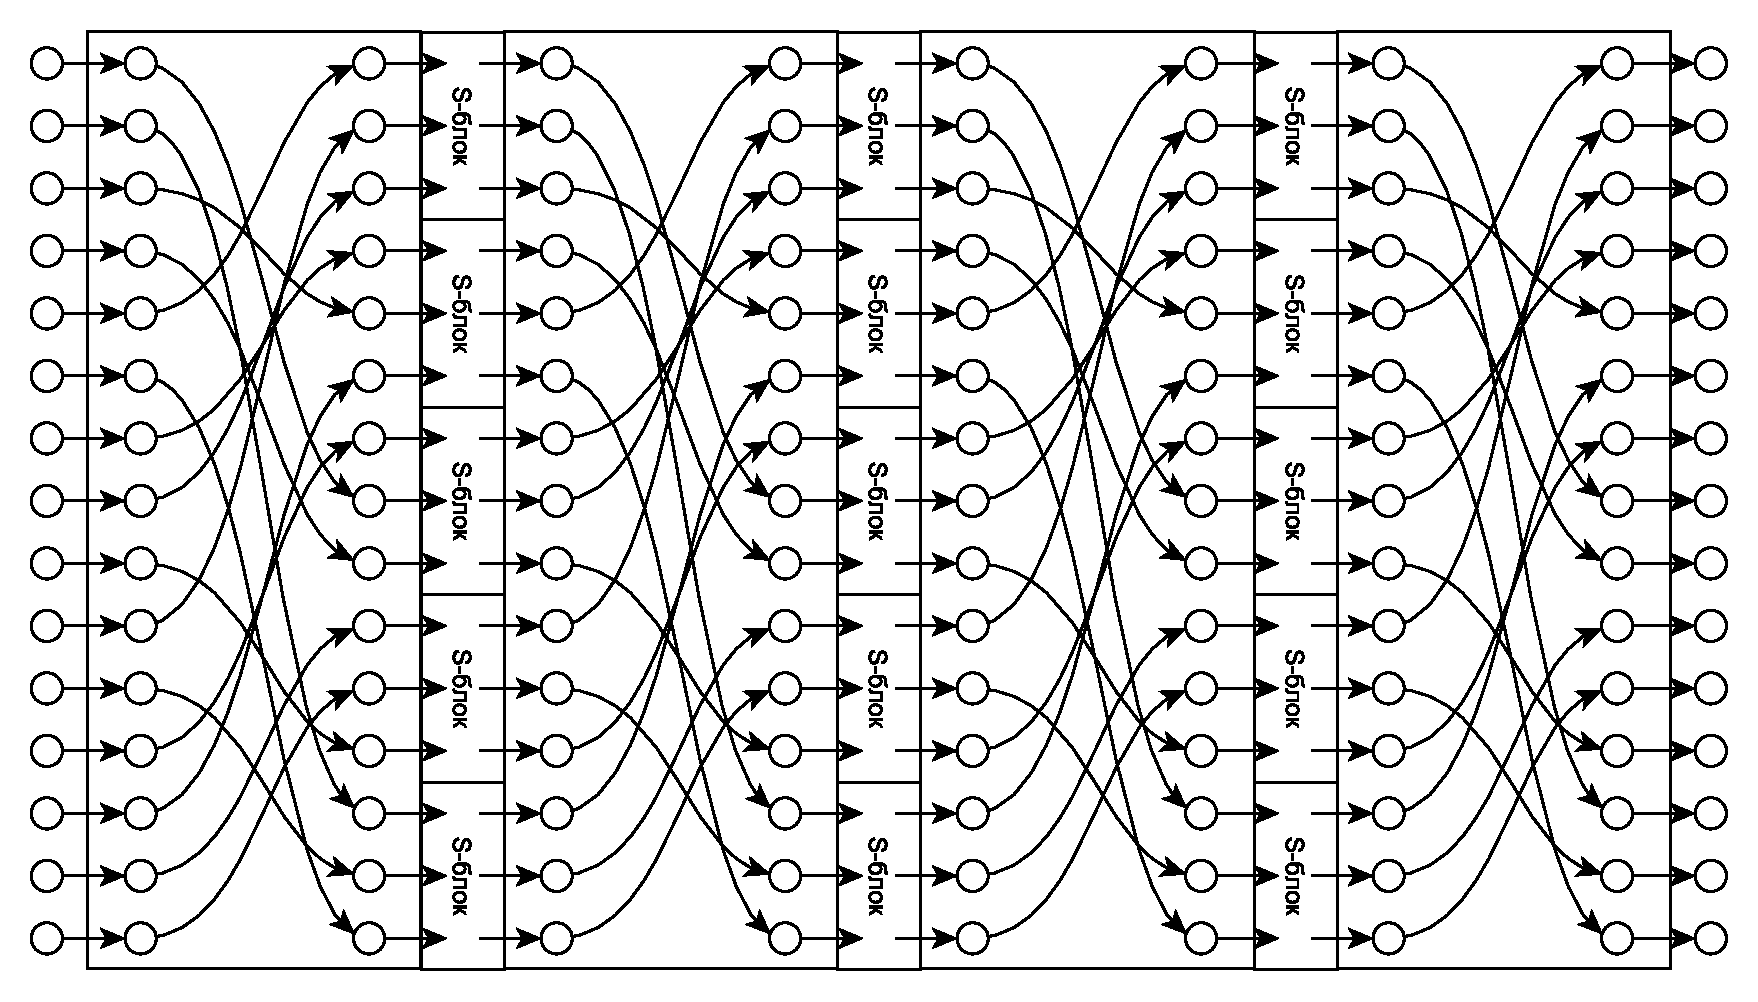
\includegraphics[width=0.8\textwidth]{pic/sp-network}
  \caption{$SP$-сеть, состоящая из 4-х $P$-блоков и 3-х слоёв $S$-блоков по 5 блоков в каждом}
  \label{fig:sp-network}
\end{figure}

Следующей составляющей будущего шифра стала возможность менять используемые $S$-блоки в зависимости от ключа. Вместо каждого из $S$-блоков в $SP$-сети Фейстель поместил модуль с двумя разными $S$-блоками. В зависимости от одного из битов ключа (своего для каждой пары блоков) использовался первый или второй $S$-блок. Результатом данного подхода стал первый вариант шифра в проекте <<Люцифер>>, который в упрощённом виде (с меньшим размером блока и меньшим числом слоёв) изображён на рис.~\ref{fig:lucifer}.

\begin{figure}[htb]
	\centering
	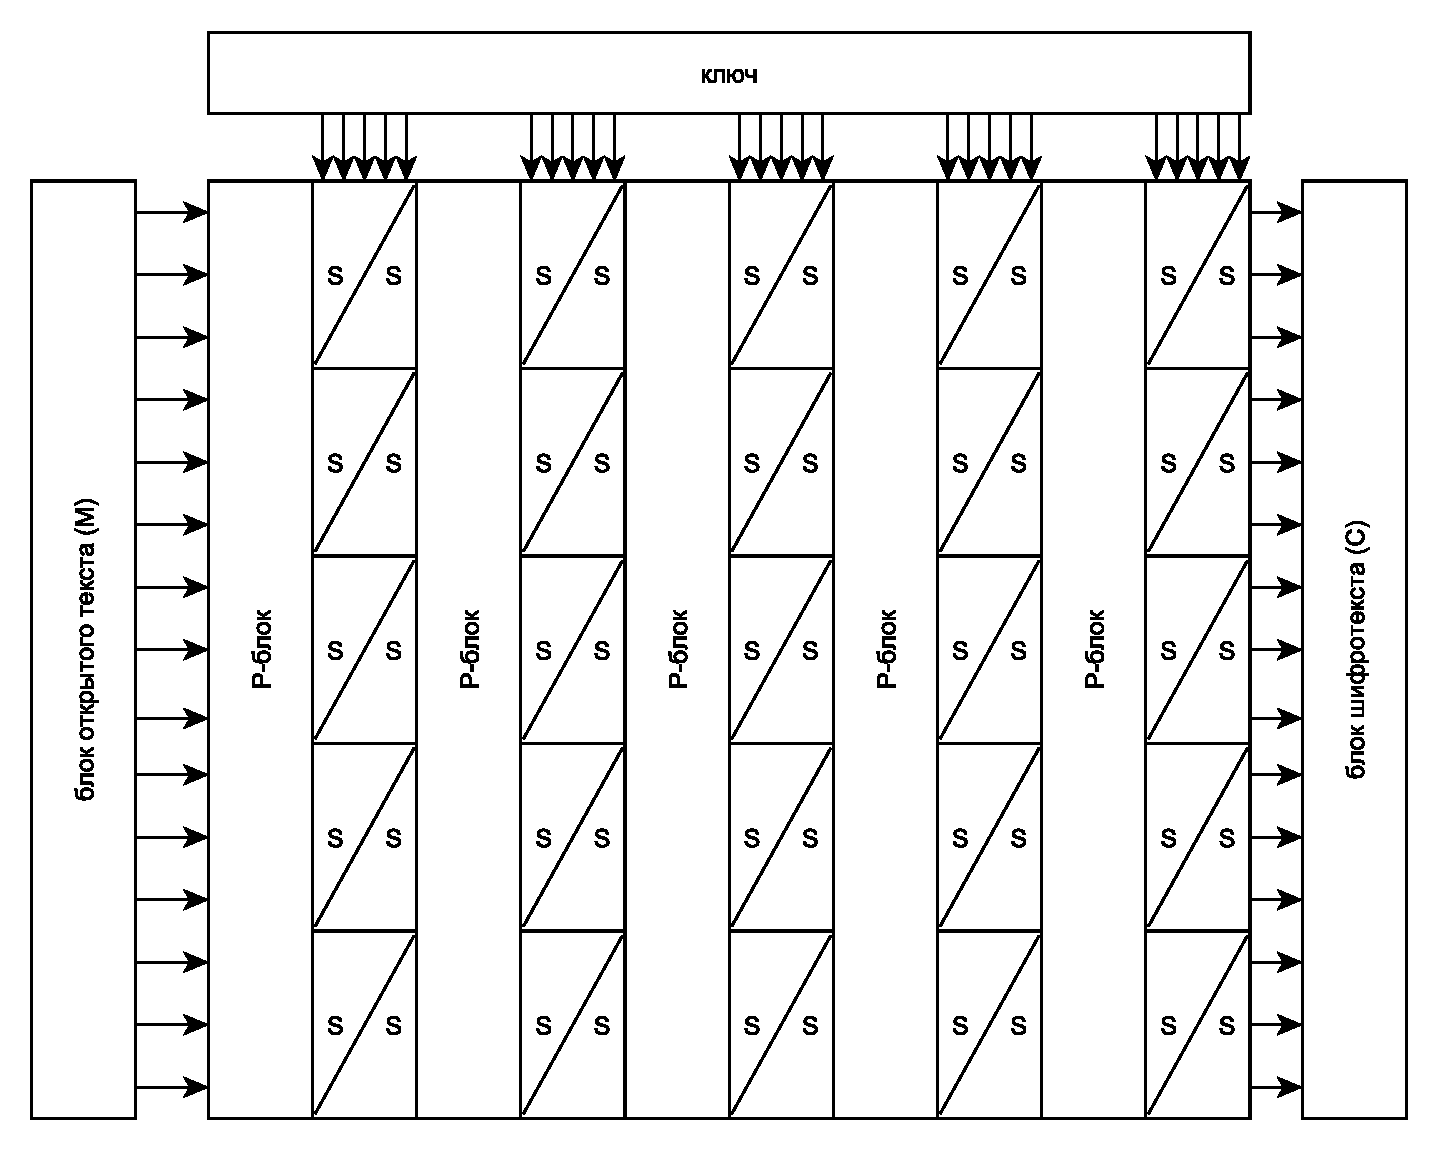
\includegraphics[width=0.8\textwidth]{pic/lucifer}
  \caption{Общий вид (упрощённая схема) функции шифрования в одном из вариантов проекта <<Люцифер>>. Входной блок (в проекте <<Люцифер>> -- 128 бит) подавался на вход на несколько слоёв (в проекте -- 16) из $P$-блоков и пар $S$-блоков. $S$-блок в каждой паре выбирался в зависимости от значения соответствующего бита ключа}
  \label{fig:lucifer}
\end{figure}\index{SP-сеть|)}

Разделение функции шифрования на относительно простые раунды (<<слои>>), комбинация больших $P$-блоков со множеством $S$-блоков малого размера -- всё это до сих пор используется в современных блочных шифрах.

\index{шифр!«Люцифер»|)}
